\subsection{Electrical Elements}

An electrical mesh analog finite difference algorithm utilizes basic circuit elements including capacitance (C), inductance (L), and resistance (R), from which more complex subsystems such RLC circuits can be designed. Redshaw and Liebmann designed an apparatus which uses the relaxation technique to solve PDEs describing oscillatory flow \cite{P.Palmer_1959} and heat transfer problems \cite{G.Liebmann_1950} using a resistive mesh.  This device, called a resistance network analogue, is comprised of resistors connected in a two-dimensional mesh configuration.  Finite difference mesh points characterize the stencil for a specific PDE, and are mapped to a resistive mesh for calculation.  Solutions are read at the intersection of resistor terminals, or nodes, as shown in Figure \ref{fig:electrical}.

\par This illustrates the resistance network analogue's ability to solve for a PDE using a voltage derived from current summation at each node.  Monitoring of the voltage at each node yields a solution for each element in the computational mesh.

\par Liebmann showed the error introduced by voltage and current measurements to be negligible, thus reducing the factors which limit the accuracy of the resistance network analogue to simply the mesh size and tolerance of components comprising the mesh~\cite{G.Liebmann_1950}.  Principles that govern the relaxation technique state that the mesh size must be made so small that the replacement of the PDE by the finite difference equation is permissible, and that any error introduced by a mismatch in mesh size and resolution requirement can be corrected with a correction function \cite{G.Liebmann_1950}.  Liebmann also showed that such a network of resistors contains averaging properties which minimize the error introduced by tolerances in individual resistor values \cite{G.Liebmann_1950}.

\subsection{Difference Equation Approximation}

\begin{figure}
\centering\fbox{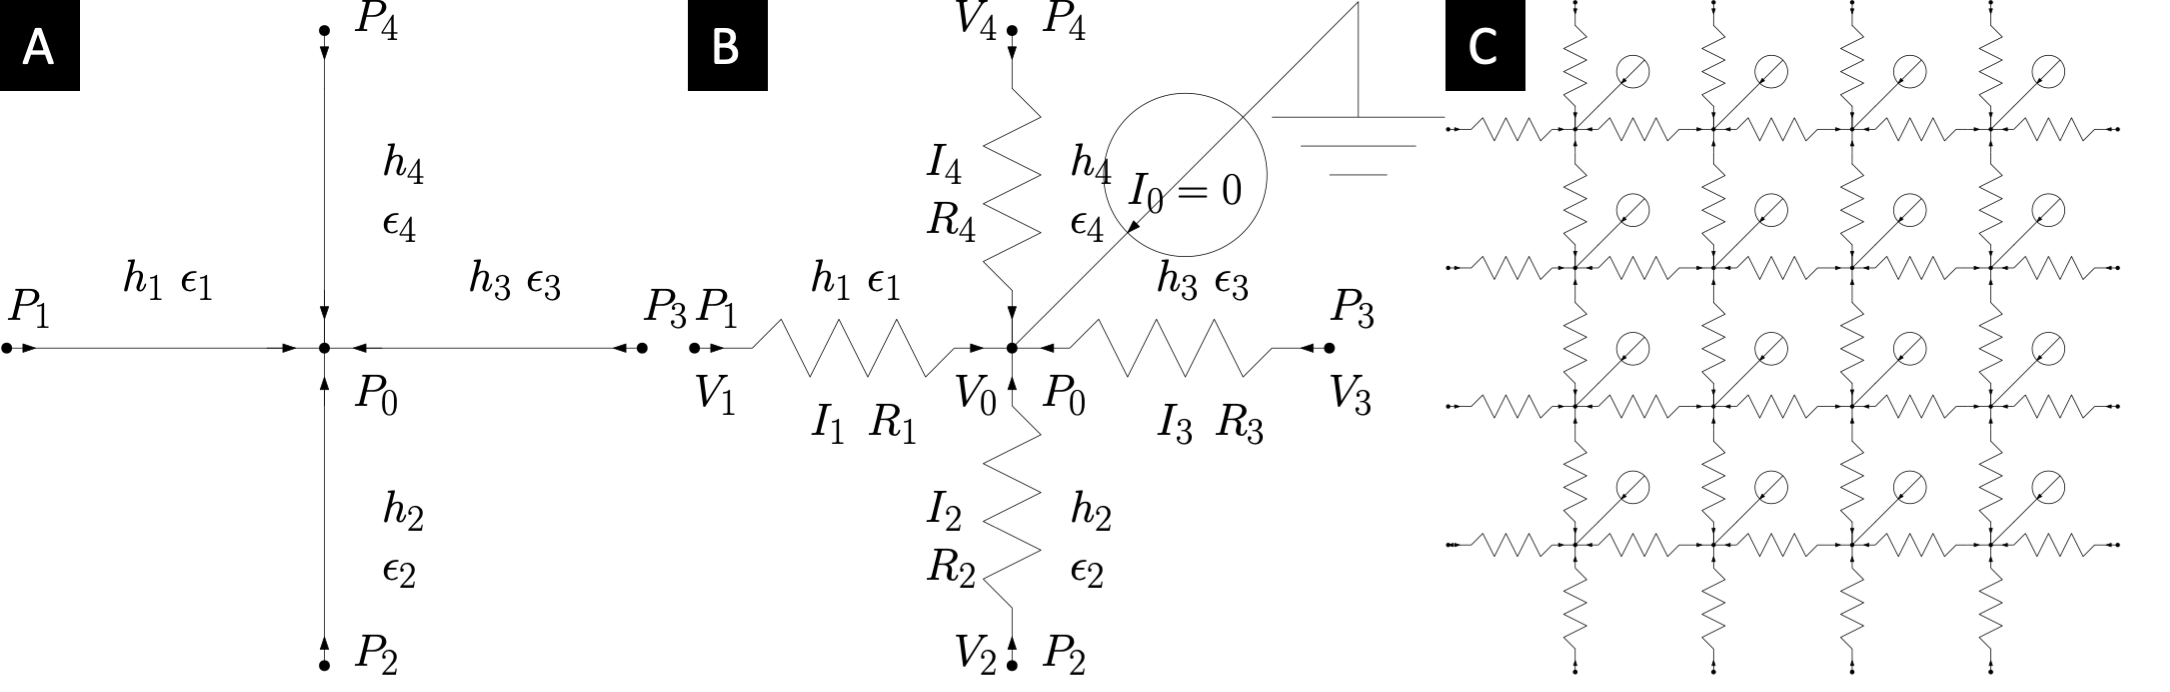
\includegraphics[height=1.5in,width=4.5in]{figures/figures2/03_finite_difference_electrical.png}}
\caption{\textbf{(A)} The derivative of the function $\varphi$ at point $P_0$ is expressed through the differences of $\varphi$ between points $P_0$ and $P_1$, $P_2$, $P_3$, and $P_4$. The distance between $P_0$ and $P_1$ is labeled $h_1$. The scalar function $\epsilon$ for vector function $\varphi$ between points $P_0$ and $P_1$, $P_2$, $P_3$, and $P_4$ is labeled $\epsilon_1$ between $P_0$ and $P_1$. \textbf{(B)}  The voltage $V$[\si{\volt}] at point $P_0$ is expressed as $V_0$. The current $I$[\si{\ampere}] and Resistance $R$[\si{\ohm}] between points $P_0$ and $P_1$ is expressed as $I_1$ and $R_1$ respectively. The same naming conventions apply for $P_2$, $P_3$, and $P_4$. $I_0$ is the input current and $R_0$ is defined in terms of other resistances, and therefor not shown on the diagram. \textbf{(C)} Poisson class electrical 16 node resistance network with the ability to apply a current at each node.}
\label{fig:electrical}
\end{figure}


\begin{equation}\label{eq:electricalLaplace_A}
  \nabla \cdot \epsilon \nabla \varphi = g 
\end{equation}

The use of an electrical mesh allows us to generate the solution of an approximation of the partial differential equation \ref{eq:supplementalElectricalLaplace} refereed to from here on as the electrical difference equation solution. In the partial difference equation \ref{eq:supplementalElectricalLaplace} where $\epsilon$ is the known scalar function, $\varphi$ is the function, and $g=0$ is  the function relationship  for a time independent Laplace second order partial differential equation. By defining an electrical mesh as shown in Figure \ref{fig:electrical} and scaling the mesh we can performing linear interpolation as shown fully in Section \ref{section:electricalDifferenceEquation} and by disregarding the higher order terms we say that Equation \ref{eq:electricalLaplace_A} is asymptotically equal to


\begin{equation}\label{eq:electricalDifferenceLaplace}
  \nabla^2 \varphi \simeq \frac{1}{h^2} \Big[ 
  \varphi\left(P_1\right) + 
  \varphi\left(P_2\right) + 
  \varphi\left(P_3\right) + 
  \varphi\left(P_4\right) -
  4\varphi\left(P_0\right)
  \Big]
\end{equation}

which is equal to

\begin{equation}\label{eq:voltageSolutionDifferenceLaplace}
  \nabla^2 \varphi \simeq \frac{1}{h^2} \Big[ V_1 + V_2 + V_3 + V_4 - 4V_0 \Big]
\end{equation}

\par The solution to the function $\varphi$ in the differential equation Equation  \ref{eq:electricalLaplace_A} has been approximated through the use of a difference equation. The solution is attained through measurement of voltage values at grid points. All that remains is to set the required boundary conditions to obtain the full solution if $g \equiv 0$ everywhere. If $g \neq 0$ currents from Equation \ref{eq:9} have to be fed into mesh points. The resistance network performs the "relaxation technique" automatically and instantaneously for a Laplace equation.

\par The accuracy of the electrical mesh pde solution is shown to increase with an increase in mesh density and be independent of the problem area size solved for between pde problem sizes 8,16,32, and 64, indicated by the reduction in the absolute (non normalized) difference between the \gls{Spice} generated electrical mesh solution script, accessible (although currently in private repository) via Section \ref{sourceCode}, and the analytical solution described in Section \ref{analyticalPDE}, and derived in Section \ref{section:pdeDerivation}, shown in Figure \ref{electricalAnalyticalDiff}. We also see that the simulation time required for the Spice circuit simulator increases exponentially for increased mesh density.

\par It is important to note that we do not have an estimate concerning the scaling of execution time of the physical electrical mesh, as we have not fabricated one, however I believe is would showcase the fundamental speedup discussed in Section \ref{bigO}. Figure \ref{electricalAnalyticalDiff} behaves in accordance with our understanding of the effects of finite difference error reduction described in Section \ref{discretizationError}.

\begin{figure}
\centering\fbox{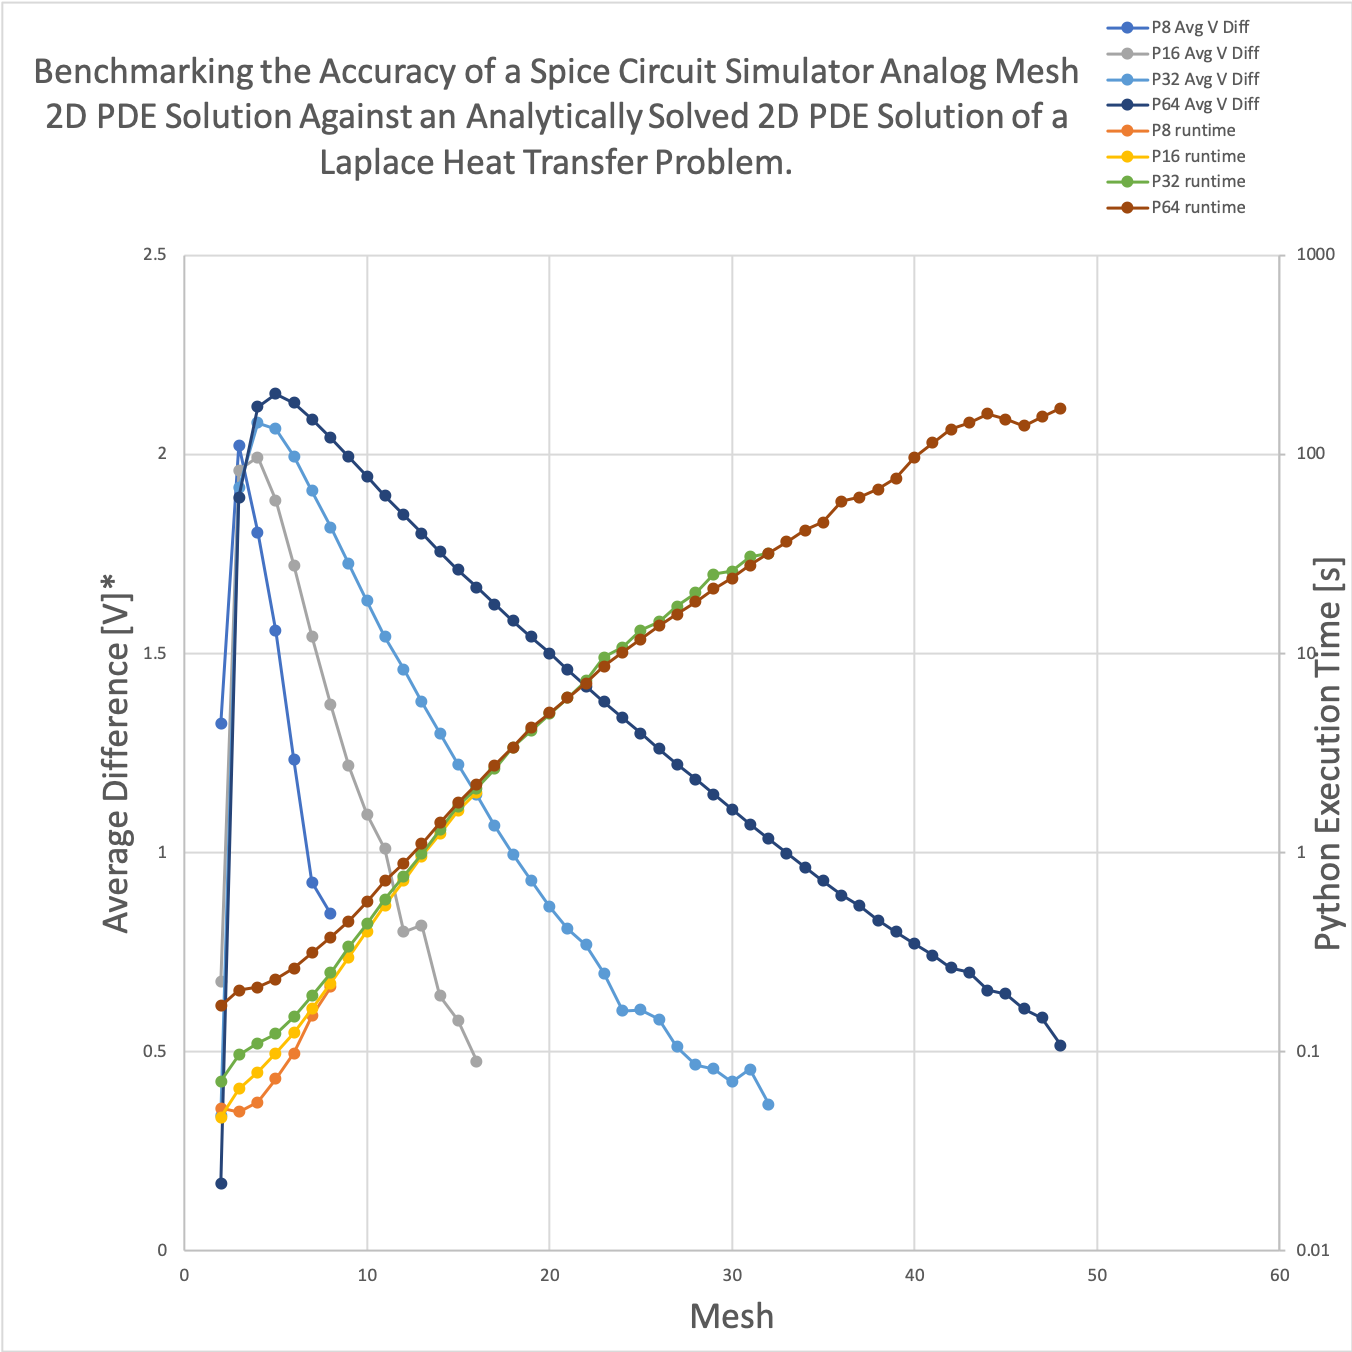
\includegraphics[height=4in,width=4in]{figures/figures2/02d_electricalDifference.png}}
\caption{Benchmarking the accuracy of a spice circuit simulator analog mesh 2D \acrshort{pde} solution against an analytically solved 2D \acrshort{pde} solution of a Laplace heat transfer problem. Mesh based solutions are scaled linearly from 2 up to the problem size N with problem sizes 8, 16, 32, and 64  plotted. Average difference is calculated by comparing the spice based voltage value at a mesh point coordinate to the value sampled from the continuous analytical solution at the same coordinate. Then the difference from all \acrfull{spice} analytical coordinate comparisons in a mesh are averaged, resulting in a single average difference point which is plotted for each mesh for each problem size. This average difference is the measure of accuracy with a higher difference resulting from a greater deviation in the spice solution from the "true north" analytical solution. Thus a lower average difference implies a higher accuracy with a value of 0 being a perfect match. *Analytical solutions not scaled for volts yet. *Program crashed at Mesh 49 on problem 64.}
\label{electricalAnalyticalDiff}
\end{figure}
